\scanpage{37}

\[
\begin{aligned}
\mathrm{Hom}^{d}(M^{*},\varphi_N N^{*})&=\mathrm{Hom}(M^{*}[-d],\varphi_N N^{*})\\
&\simeq\mathrm{Hom}(\tau_N(M^{*}[-d]),N^{*})\\
&\simeq\mathrm{Hom}((\tau_{N-d}M^{*})[-d],N^{*})\\
&\simeq\mathrm{Hom}^{d}(\tau_{N-d}M^{*},N^{*})
\end{aligned}
\]

\margin{$N^{*}\in\mathrm{Ob}\,\mathcal{M}_N$}

\[
\boxed{\mathrm{Hom}^{d}(M^{*},\varphi_N N^{*})\simeq\mathrm{Hom}^{d}(\tau_{N-d}M^{*},N^{*})}
\]

\uline{Supposons} $M^{*}\in\mathcal{M}^{*}_{\deleted{\unsure{d}}-d}$ $[\text{i.e. } M^{j}=0\text{ si }j<-d]$,

\[
\begin{aligned}
\mathcal{N}^{*}&=\tau_N N\otimes_k S_k\deleted{\unsure{=}}=\tau_N\mathcal{N}_{S_k}\quad (N\text{ un }k\text{-module})\\
&\quad N\geq 0
\end{aligned}
\]

\[
\begin{aligned}
\text{Alors }\quad\mathrm{Hom}^{d}(M^{*},\varphi_N\tau_N\mathcal{N}^{*}_{S_k})
&=\mathrm{Hom}^{d}(M^{*},\underbrace{\varphi_{\unsure{\infty N|N}}\tau_N\mathcal{N}^{\unsure{\alpha|*}}_{S_k}}_{=\tau_N\varphi_N\tau_N\mathcal{N}^{\unsure{*|s}}_{S_k}})=\mathrm{Hom}^{d}(M^{*},\tau_N\\
&=\unsure{\mathrm{H}}
\end{aligned}
\]

\figure{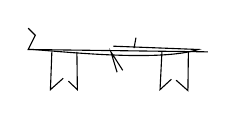
\begin{tikzpicture}[x=6mm,y=6mm]
\draw (0,.5)--(.15,.35)--(0,.05)--(3.8,0);
\draw (.1,.05) .. controls (1,-.02) and (2.8,-.2) .. (3.6,.05) -- (1.8,.12);
\draw (.5,0)--(.47,-.8)--(.74,-.56) (1.03,0)--(1.04,-.8)--(.85,-.62)
 (1.88,-.43)--(1.75,0)--(2,-.39) (2.28,.3)--(2.24,.08)
 (2.83,0)--(2.79,-.8)--(3.03,-.58) (3.39,0)--(3.38,-.82)--(3.13,-.6);
\end{tikzpicture}}

% The following cancelled block is written upside down.

\deleted{\[
\boxed{G,\quad g_1,\quad\ \ ,g_r}\quad
\begin{gathered}\longrightarrow\\[-2pt]\twoheadrightarrow\end{gathered}
\]

Diagramme de Cayley

\diagram{\begin{tikzcd}[ampersand replacement=\&,row sep=5mm,column sep=7mm,
execute at end picture={
\begin{scope}[shift={(\tikzcdmatrixname-2-2.center)},x=1cm,y=1cm]
\draw (0,0) .. controls (0,1.9) and (1.85,2.8) .. (3.05,1.9) .. controls (4,1.2) and (1.65,.65) .. (0,0);
\draw[->] (0,0)--(.04,.46);\draw (.04,.46)--(.09,1);
\draw (0,0)--(1.42,.98);\draw[->>] (0,0)--(.38,.22);
\draw[->>] (.09,1)--(.63,1.2);\draw[->>] (0,0)--(.34,-.36);
\draw (-.22,-.42)--(0,0);
\fill (.09,1) circle(1.8pt) (1.42,.98) circle(1.5pt) (0,0) circle(1.8pt);
\node[below] at (.05,0) {$x$};\node[right] at (1.36,.75) {$xg_i$};
\fill (-1.45,.03) circle(1.2pt) (-1.38,-.27) circle(1.2pt) (1.55,0) circle(1pt) (3,0) circle(1.2pt) (4.65,-.13) circle(1pt);
\draw (4.68,-.34) .. controls (6.1,-.1) and (7.8,-.2) .. (7.12,1.23);
\node[below] at (4.71,-.33) {$\unsure{y|g}$};
\draw[thin] (-.67,1.98)--(1.76,-1.63) (3.1,2.25)--(5.85,-1.78);
\end{scope}}]
\vphantom{x}\&\vphantom{x}\\
\vphantom{x}\&\vphantom{x}
\end{tikzcd}}

Mot en les $g_i$ $+$ origine

$g,\ g_i$}

% archive sheet number: 36
